The third prototype built and the first thought to be the final version of the TRITIUM detector module was Tritium-Aveiro 0, shown in figure \ref{fig:TritiumAveiro0}, which was designed and built in the Aveiro workshop. 

\begin{figure}[h]
\centering
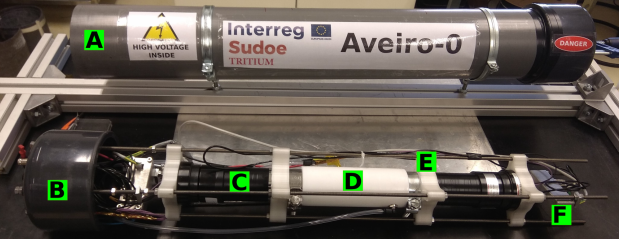
\includegraphics[scale=0.4]{5Prototypes/53FinalPrototypes/531TritiumAveiro/GeneralViewOfAveiroPrototype.png}
\caption{Tritium-Aveiro prototype.\label{fig:TritiumAveiro0}}
\end{figure}


It consists of a teflon vessel (D of figure \ref{fig:TritiumAveiro0}), shown in figure \ref{fig:TeflonStructureFibersTritiumAveiro0}, which has an internal cylindrical hole whose diameter and length are $43~\mm$ and $180~\mm$ respectively. 

\begin{figure}[h]
\centering
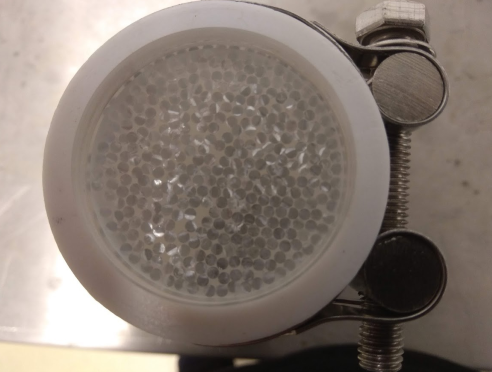
\includegraphics[scale=0.4]{5Prototypes/53FinalPrototypes/531TritiumAveiro/TeflonVessel_Fibers.png}
\caption{Teflon structure and fiber bundle used in Tritium-Aveiro 0 prototype.\label{fig:TeflonStructureFibersTritiumAveiro0}}
\end{figure}

This vessel contains $360$ no-clad scintillating fibers with a length of $180~\mm$. The model of the used fibers is BCF-10 from Saint-Gobain company \cite{DataSheetBCF10Fiber}, which have practically the same characteristics than the others used up to now (BCF-12 fibers) and its most important difference is the diameter, which is the double, $2~\mm$.

On the one hand, a larger diameter could be interesting because it facilitates the flow of water around the fibers, reducing the problems related to surface tension and ensuring that the entire active volume of the fibers is used for tritium detection. In addition, it increase the resistance of the fibers, which is very important since the water is flow around them.

On the other hand, a larger diameter could be detrimental since it worsens the signal-to-background ratio. It happens because, with $2~\mm$ fibers, the active volume that our detector has in the same space is smaller so its signal will be smaller and the part of the fibers where no tritium events reach (they only contribute to the background) is larger so the background will be larger.

In order to quantify the importance of the effect of the fiber diameter, which is needed to choose the best configuration, these measurements will be compared with similar measurements performed with Tritium-IFIC 2 prototype which, as we will see in next section, is based on a similar configuration with $1~\mm$ fibers (BCF-12 model).

The amount of fibers used in Tritium-Aveiro 0 prototype is the maximum which allows the water to flow and, due to the large quantity of fibers used, these fibers are not feasible to use any structure to fix them. It should be noted that these fibers were cut with the fiber cutting device developed by TRITIUM but they were neither polished nor cleaned. The reason for this is that the automatic polishing machine was not yet developed and it was not feasible to polish 360 fibers by hand. In fact, the automatic polishing machine was motivated by the amount of fibers used in our last prototypes.

To ensure the radiosecurity of this prototype, the teflon vessel is totally closed and it has two PMMA windows, whose thick is $10~\mm$, located at both ends of the fiber bundle which will be used to read it. Two clamps are used to press the Teflon walls against the PMMA windows to ensure the watertightness of the prototype.

PMMA was chosen for its optical properties, especially its transmission coefficient, which was measured for visible light range in the ICMOL laboratories and it is shown in the figure \ref{fig:PMMATransmissionSpectrum}.

\begin{figure}[h]
\centering
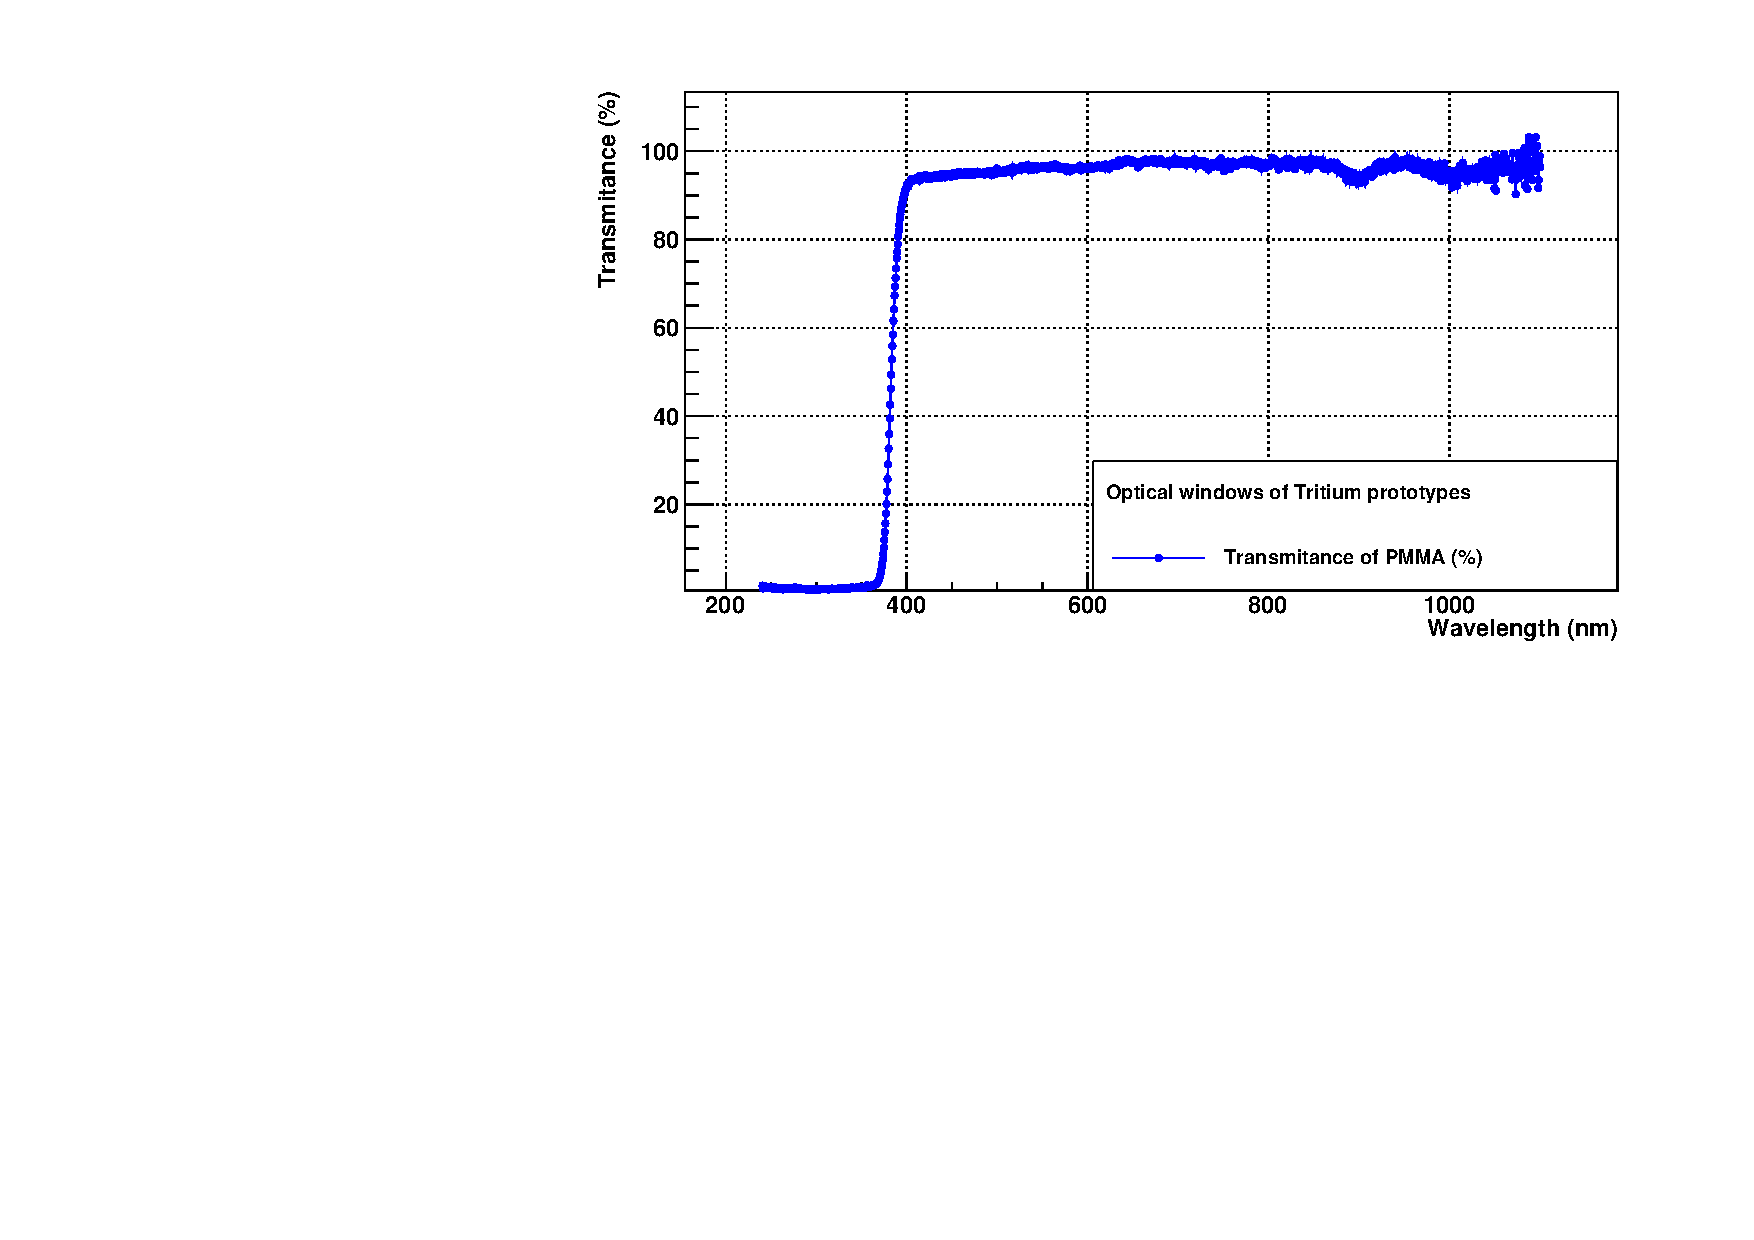
\includegraphics[scale=0.6]{5Prototypes/53FinalPrototypes/531TritiumAveiro/TransmissionSpectrumPMMA_cut_at_low_energy.pdf}
\caption{Transmission spectrum of light (in the visible range) in a piece of PMMA of X thickness measured in the ICMOL laboratory. \label{fig:PMMATransmissionSpectrum}}
\end{figure}	

As can be seen, its transmission coefficient is $95\%$ for the working wavelength ($435~\nm$), which means that the loss of the light in these optical windows is very small. Slightly better transmission coefficients can be achieved with other materials such as quartz or sapphire but they are much more expensive.

Two PMTs (C of figure \ref{fig:TritiumAveiro0}), powered at $-1500~\volt$, are used to read this prototype in time coincidence. They are fixed to both fiber bundle ends of the prototype using two pieces (E of figure \ref{fig:TritiumAveiro0}) which has been designed and built with a 3D printer. Both PMTs are optically coupled to the PMMA windows using optical grease \cite{OpticalGrease}.

The PMTs used are the model R2154-02 2" from Hamamatsu company \cite{DataSheetPMTsAveiro}, whose characteristics, specially its gain and efficiency, are quite similar to the PMTs used in the other prototypes.

All these different parts, together with the electronic system (F of figure \ref{fig:TritiumAveiro0}), is arranged in a structure, seen in figure \ref{fig:TritiumAveiro0}, which is based on several nuts located on four long stainless-steel screws. This screws are fixed to an external PVC structure, A and B of figure \ref{fig:TritiumAveiro0}, which is used to protect the prototype from physical damage and provide a light-tight operation environment. This PVC structure is equiped with several high voltage power, low voltage power and signals feed-through connectors.

Only one prototype was built, which was designed to be installed in the Arrocampo dam. To do so, on the one hand, a water inlet/outlet were installed in its Teflon vessel to allow a constant water flux through the detector and, on the other hand, several PCBs was specially designed, developed and tested to process and analyze the signals of this system.

On the one hand, a PCB, whose electronic scheme is shown in figure \ref{fig:HVElectronicAveiro}, was designed to power the PMTs with a negative high voltage. It consists of several high voltage power supply, model C11152-01 from Hamamatsu company \cite{PowerSupplyAveiroDataSheet}, one for each PMT used, which is controled by a DAC\footnote{DAC, Digital-to-analog converter}, model MAX5500 from Maxim Integrated company \cite{MAX5500DataSheet}. An Arduino Mega is used for the DAC communication and cross-checking the output values and it is connected to a Raspberry Pi to control the system.

A graphical interface, shown figure \ref{subfig:GUI}, has been developed to manage the different options of this system in a comfortable way.

\begin{figure}[h]
 \centering
  \subfloat[Electronic scheme of the PCB]{
   \label{subfig:ElectronicSchemeHVBoard}
    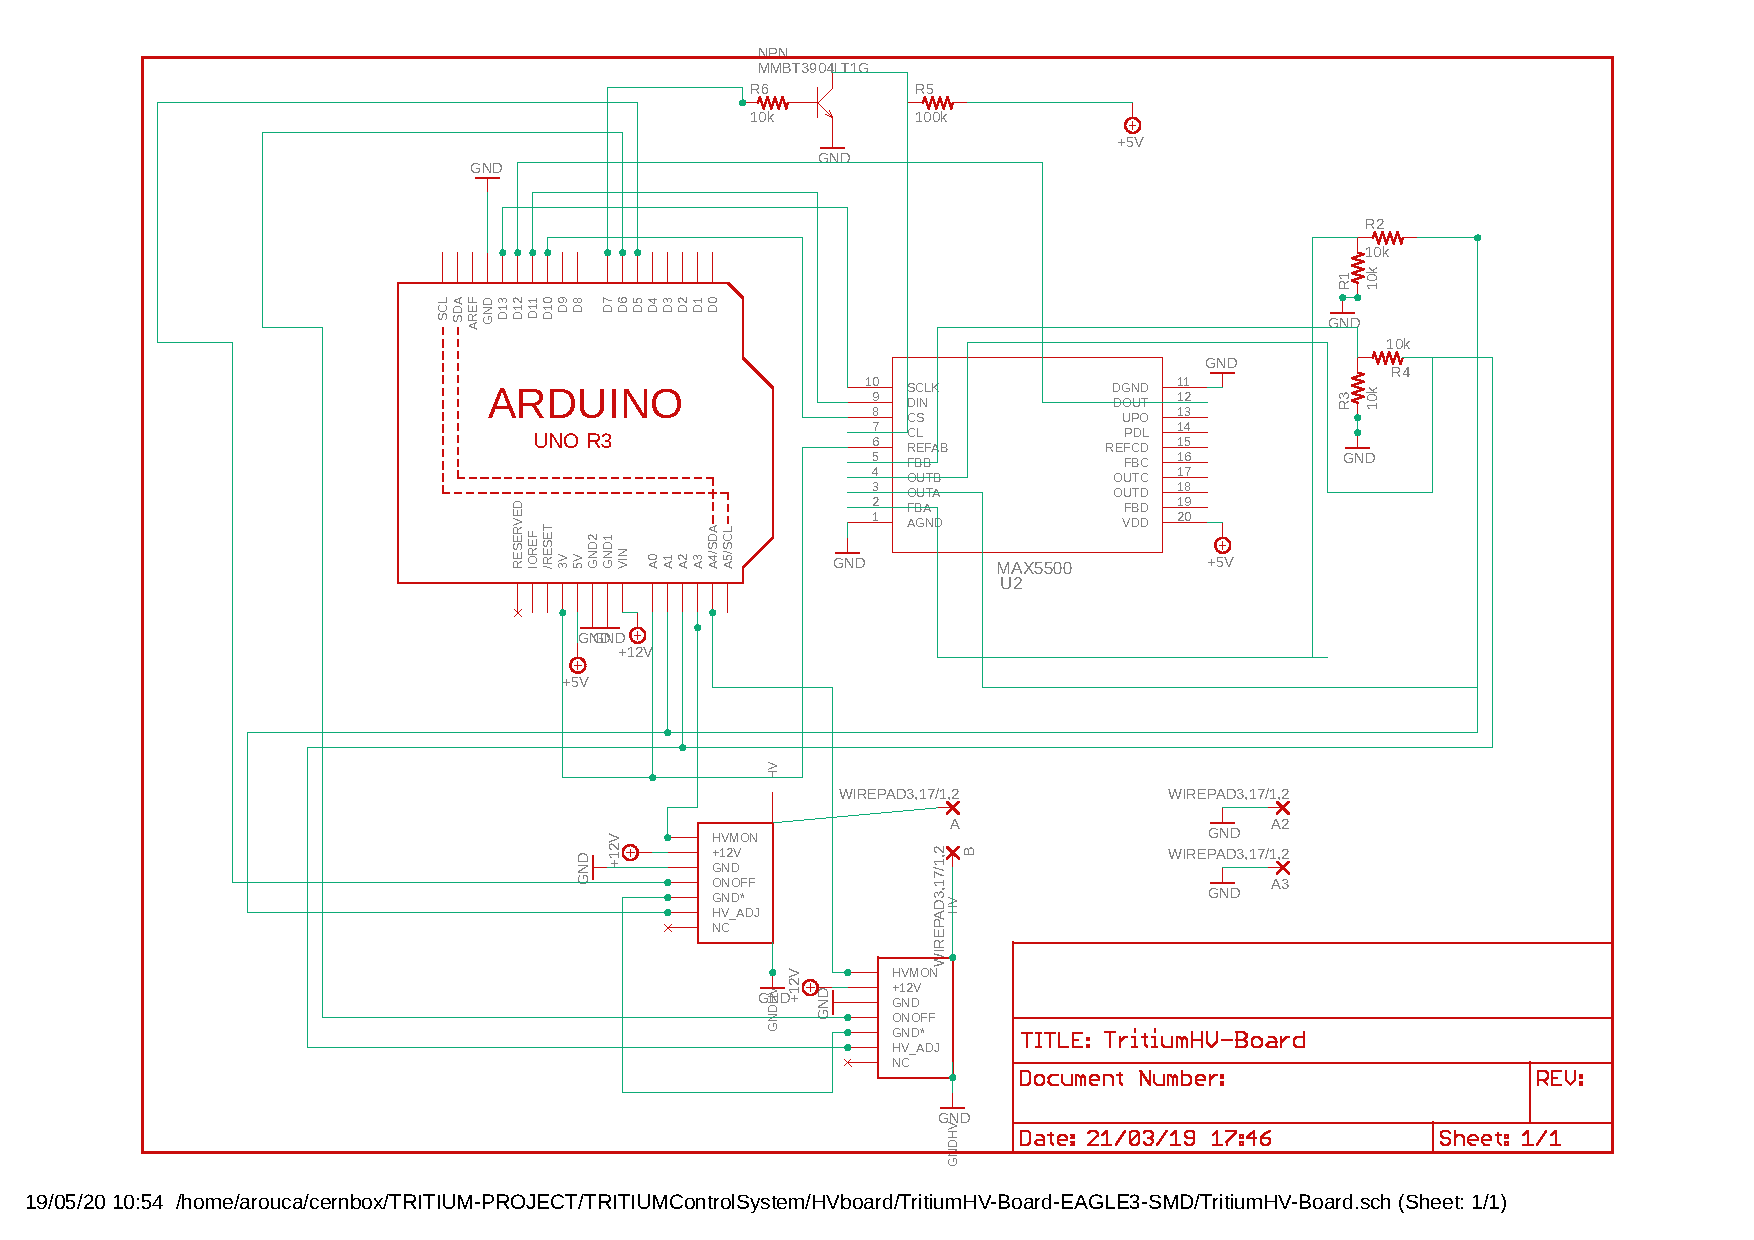
\includegraphics[angle=0, width=0.5\textwidth]{5Prototypes/53FinalPrototypes/531TritiumAveiro/TritiumHV-Board.pdf}}
    %\newline
  \subfloat[Graphical user interface]{
   \label{subfig:GUI}
    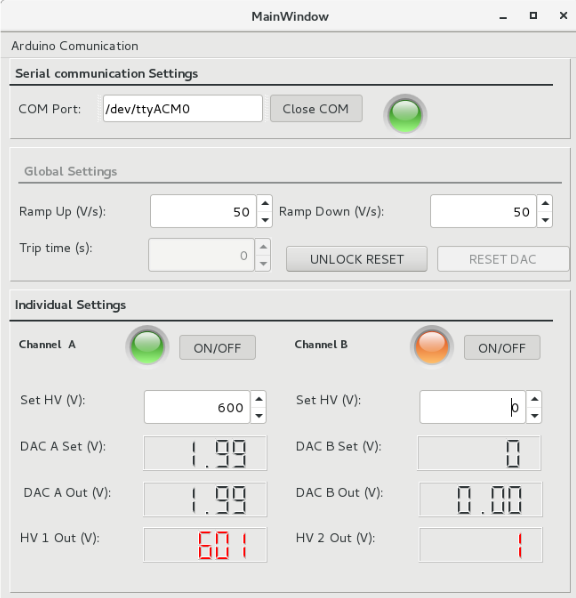
\includegraphics[angle=0, width=0.5\textwidth]{5Prototypes/53FinalPrototypes/531TritiumAveiro/GUIHVBoard.png}}
 \caption{Electronic scheme of the PCB designed to power the PMTs of Aveiro prototype and the graphical user interface developed to control it.}
 \label{fig:HVElectronicAveiro}
\end{figure}

On the other hand, a electronical chain consisting of several PCBs was used to process and analyze the system signals, whose simplified electronic scheme is shown in figure \ref{fig:ElectronicSchemCounterBoard}.

\begin{figure}[h]
\centering
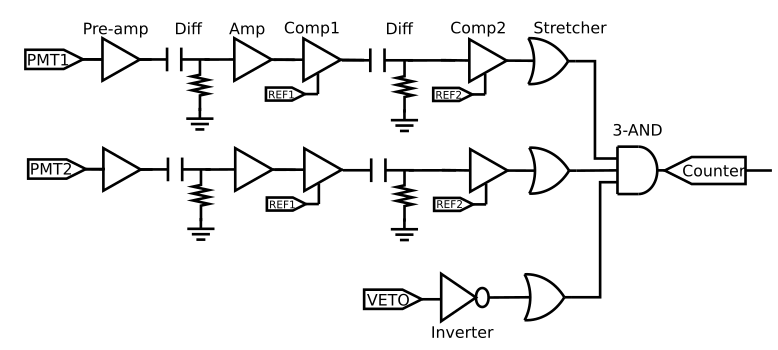
\includegraphics[scale=0.45]{5Prototypes/53FinalPrototypes/531TritiumAveiro/ElectronicSchemeCounterBoard.png}
\caption{Simplified electronic scheme used to process and analyze the signal of Tritium-Aveiro 0 prototype. \label{fig:ElectronicSchemCounterBoard}}
\end{figure}

It consists of three different lines, two of them are used for the PMT signals of the prototype and the remaining line is used for doing anticoincidence with a active veto.

To test this electronic chain a plastic scintillation with dimensions of $10 \cdot{} 10 \cdot{} 1~\cm^3$ was used to simulate a veto signal but four different vetos are being developed, each one is based on a rectangular plastic scintillations of Saint-Gobain company \cite{VetoAveiro}, whose dimensiones are $50~\cm \cdot{} 30 \cdot{} 2~\cm^3$  with a PMT coupled, model R2154-02 2" from Hamamatsu company \cite{DataSheetPMTsAveiro}. The output signal of these PMTs will be input in a OR stage, whose response will be introduced in the veto line shown previously in the figure \ref{fig:ElectronicSchemCounterBoard}. As a result, each plastic scintillator will be read in anticoincidence with tritium-Aveiro prototype.

Both lines, used to process and analyze the PMT signals of the prototype, are equal and they are used to operate in time coincidence. First, each PMT signal is introduced in a prepamplifier model CR111 from CREMAT Inc. company \cite{CREMATPreAmplifierDataSheet}, which is used to shape and pre-amplify the signal. To reduce electronic noise and signal loss, both preamplifiers are connected as close as possible to the PMTs and they are located inside of aluminum boxes which act like a Faraday cage.

Each preamplifier is followed by a differentiation stage, which is used to reduce the time width of the signal, and amplification stages, used to amplify the signal. The amplification used is the model OPA656 from Texas Instruments \cite{OPA656}. 

Then, a fast comparator, model LT111 from Linear Technology company \cite{LT111}, is used to set a threshold which will be used to remove the PMT signals whose amplitude are below this value (dark counts of the PMT). A MAX5500 DAC is used to configure the thresholds.

The time width of the preamplfier output signal is too large, $200~\mu\second$, so which too many false coincidence will be registed. To solve this problem a second differenciation stage is included and a second comparator are added to produce a 5V square signal again.

Finally a tunable pulse stretcher based on an OR gate, model SN74AHC1 from Texas Instruments company \cite{Stretcher}, is used to set the time width of each signal at $100~\nano\second$, with which the time coincidence windows of our adquisition system is $200~\nano\second$, narrow enough to have a negligible false coincidence rate.

In the remaining line, used for the veto signal, an inverter is used in the first stage. With it, the signal will always be in the high level, $5~\volt$, except when a cosmic particle is detected, in which case the signal will be in the low level, $0~\volt$. Then, another stretcher is used to create a signal with the same time width than the others, $100~\nano\second$.

Lastly, these three signals are introduced into a 3-input AND gate, model SN74LVC1G11 from Texas Instruments company \cite{ANDGate}, to perform a logic level comparison. With this last stage we achieve a temporal coincidence of both PMT signals of the prototype and anti-coincidence of them with the veto signal. The output signal of this last stage is simply connected to a pulse counter. 

A GPIO pins of a Raspberry Pi is used to communication with the system, control it and configure the different threshold levels and a graphical user interface, whose appearance is shown in figure \ref{fig:GUIcounts}, has been developed to manage in a comfortable way the counter system.

 \begin{figure}[h]
\centering
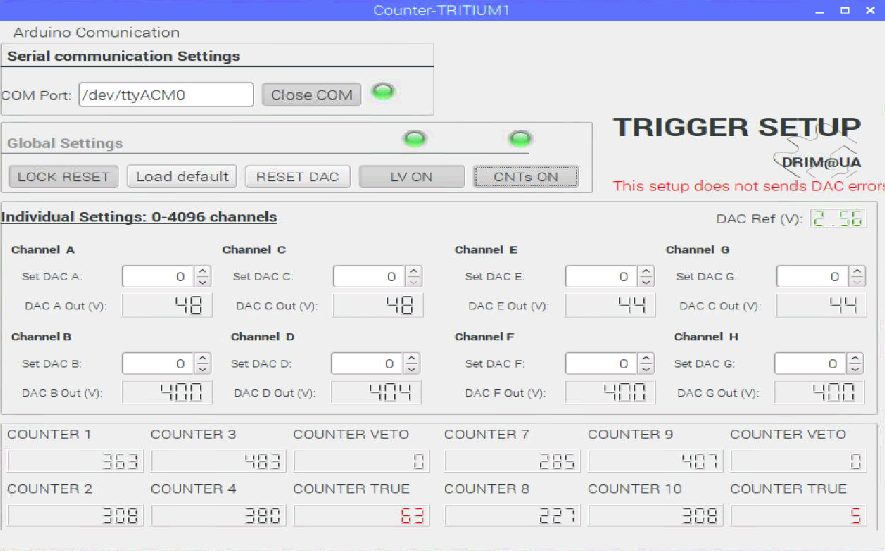
\includegraphics[scale=0.45]{5Prototypes/53FinalPrototypes/531TritiumAveiro/CounterGUI.png}
\caption{Graphical user interface used to manage the counter system. \label{fig:GUIcounts}}
\end{figure}

In addition to count, which is the option normally used in our detector, this electronic system include a voltage follower circuit connected to the preamplifier output signal which can be used to obtain a energy spectrum of each PMT of the prototype.

It is important to note that, although this system has a graphical user interface that allows comfortable control of the system, the usual way in which it is controlled is remotely through the computer terminal.

In the figure \ref{fig:ScreenshotElectronic} two screenshots are shown to demostrate two different situations of this system. There, we have four different signals. The yellow and cyan signal are input signals of the AND-Gate, which come from the PMT signals of the prototype. The pink signal is the third remaining input signal of the AND-Gate, which come from the PMT signal of the veto. The last signal, green, is the output signal of the AND-Gate.

\begin{figure}[h]
 \centering
  \subfloat[Event accepted by the electronic system]{
   \label{subfig:TrueTritiumEvent}
    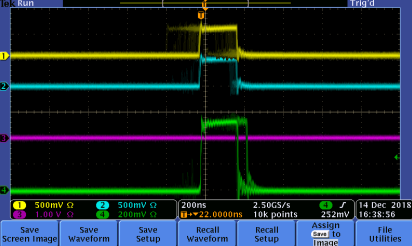
\includegraphics[angle=0, width=0.42\textwidth]{5Prototypes/53FinalPrototypes/531TritiumAveiro/Event_accepted_Aveiro_prototype.png}}
    %\newline
  \subfloat[Event rejected by the electronic system]{
   \label{subfig:FalseTritiumEvent}
    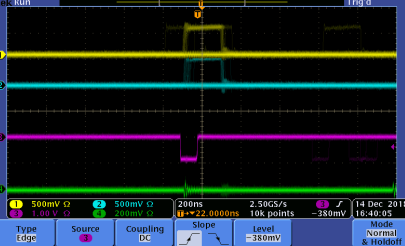
\includegraphics[angle=0, width=0.42\textwidth]{5Prototypes/53FinalPrototypes/531TritiumAveiro/Event_rejected_Aveiro_prototype.png}}
 \caption{Two different situations of the electronic chain response. A.- Event accepted since veto has not detected it. B.- Event rejected since veto has detected it}
 \label{fig:ScreenshotElectronic}
\end{figure}

As can be seen, in the figure \ref{subfig:TrueTritiumEvent} both PMTs of the prototype have detect a time coincident event, which has not been detected for the veto, so this event is counted. In the figure \ref{subfig:FalseTritiumEvent}, a time coincidence event has been observed in the three PMTs, which means that it is a cosmic event, so this event is not counted.

First some measurements were taken in the laboratory that were used to characterize the detector. For this task is was filled with ultra-pure water, which was used to measure the background of the detector, and then, it was filled with several radioactive liquid tritium solutions with different activities, $10~\kilo\becquerel/\liter$ and $30~\kilo\becquerel/\liter$, which were used the mesure the efficiency and the sensitivity of this module.

Later, it was installed in the arrocampo dam to test its functionality and to begin with the tritium level monitoring.

All this measurements will be shown in the section \ref{subsec:ResultsTritiumAveiro}, where it will be discussed and compared with the measurements of the previous prototypes.

%La eficiencia máxima del fotocátodo (26\%) ocurre para la longitud de onda de 420 nm, figura 3.2.a,